%!TEX root = ./template-skripsi.tex
%-------------------------------------------------------------------------------
%                            BAB III
%               		METODE PENELITIAN
%-------------------------------------------------------------------------------

\chapter{METODE PENELITIAN}

\section{Deskripsi Sistem}
    Sistem yang akan dibuat pada penelitian ini adalah sistem yang dapat melakukan pelacakan pergerakan objek ikan dengan menggunakan metode GMM dan Kalman Filter. Fokus dari penelitian ini adalah untuk menghasilkan \textit{output} berupa video yang di dalamnya terdapat objek yang sudah dilacak lengkap dengan \textit{bounding box} serta label uniknya. Dataset video yang akan digunakan pada sistem ini berasal dari dua sumber. Sementara bahasa pemrograman yang digunakan untuk membuat sistem adalah Python versi 3. 
    
    Tahapan proses pelacakan pergerakan objek ikan dengan menggunakan metode GMM dan Kalman Filter adalah memasukan \textit{input} video, deteksi objek bergerak dengan GMM, \textit{noise removal} dengan \textit{Morphology Operation}, \textit{Contour Tracing}, \textit{tracking} masing-masing objek menggunakan Kalman Filter, \textit{decision of occlusion}, dan terakhir adalah tahap asosiasi data. Tahapan-tahapan tersebut akan terus berulang selama video berlangsung.
    
\section{Perancangan Sistem}
    Bagian ini membahas tentang desain proses yang digunakan untuk mengetahui tahapan-tahapan yang dilakukan untuk membangun sistem pelacakan pergerakan objek ikan. Tahapan tersebut adalah sebagai berikut: tahap \textit{input} video yang kemudian dibaca oleh sistem dalam bentuk citra (\textit{frame} per \textit{frame}). Lalu dilakukan proses deteksi objek ikan yang bergerak menggunakan GMM, setelah itu dilakukan proses \textit{Morphology Operation} untuk menghilangkan \textit{noise} dari proses deteksi objek menggunakan GMM. Kemudian teknik \textit{downsampling} dan \textit{contour tracing} dijalankan untuk menghasilkan \textit{border} dari piksel yang dapat dikatakan sebagai objek. \textit{Bounding box} kemudian dipasangkan kepada masing-masing objek tersebut dan \textit{decision of occlusion} dilakukan. Terakhir Kalman Filter diinisiasi atau diperbarui untuk setiap objek yang ada. Hal ini dilakukan untuk memasangkan atau mempertahankan label unik masing-masing objek sehingga objek dapat terus dilacak atau diasosiasikan dengan tepat selama video berlangsung. Keluaran yang dihasilkan adalah sebuah \textit{running} video yang di dalamnya terdapat objek-objek yang sudah dilacak lengkap dengan label unik serta \textit{bounding box}-nya.
    \begin{figure}[H]
    \centering
      \singlespacing
      \captionsetup{justification=centering,margin=0.5cm}
      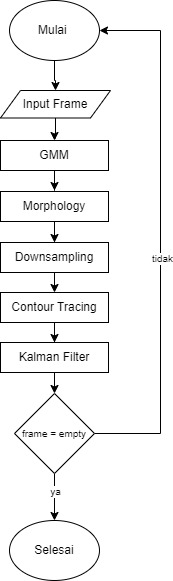
\includegraphics[width=4cm]{image/system-flow-chart.jpg}
      \caption{Diagram alir keseluruhan proses sistem}
      \label{fig:overalfc}
    \end{figure}
    
    \subsection{Proses Input Video}
        Data yang digunakan sebagai masukan dari sistem adalah video dengan format .mp4 atau .flv. Masukan video dibaca ke dalam bentuk citra sehingga menghasilkan \textit{frame} video. Setiap \textit{frame} video juga melalui proses \textit{pre-processing} dahulu sebelum masuk ke tahap deteksi objek dengan metode GMM yaitu, mengubah ruang warna citra dari RGB ke \textit{grayscale} .
        
    \subsection{Keluaran}
        Keluaran yang diharapkan dari sistem  adalah \textit{running} video yang di dalamnya sudah terdapat objek yang dilacak menggunakan metode GMM dan Kalman Filter lengkap dengan \textit{bounding box} serta label unik yang mengikutinya.
        
    \subsection{Deteksi Objek dengan GMM}
        Metode yang digunakan untuk mendeteksi objek ikan bergerak pada video adalah \textit{Background Subtraction} dengan bantuan GMM untuk memodelkan latar belakangnya. Langkah pertama pada GMM adalah inisialisasi Gaussian $\eta$ untuk memodelkan nilai piksel pada observasi $X_1$ dengan $\omega = 1$, $\mu = X_1$, dan varians $\sigma$. Observasi $X_1$ adalah observasi nilai sebuah piksel pada waktu $t$.
        
        Selanjutnya, setiap piksel baru $X_t$ akan diperiksa terhadap $K$ distribusi Gaussian yang sudah ada sampai terdapat \textit{"match"}. Sebuah piksel dapat dikatakan \textit{"match"} jika nilai piksel tersebut terletak dalam jangkauan 2,5 dari nilai standar deviasi sebuah distribusi. Jika terdapat \textit{"match"} maka parameter $(\omega, \mu, \sigma)$ dari distribusi Gaussian tersebut diperbaharui. \textit{Learning rate} $\alpha$ merupakan parameter dari sistem. Jika tidak terdapat \textit{"match"}, maka distribusi lama yang mempunyai nilai kemungkinan paling kecil akan digantikan oleh distribusi baru. Distribusi  baru  ini  menggunakan  nilai  piksel  baru  sebagai  rata-rataanya, memiliki nilai varians awal yang besar, dan juga bobot yang rendah.\\
        
        Distribusi $K$ kemudian diurutkan berdasarkan nilai $\omega/\sigma$ dari masing-masing distribusi dan distribusi $B$ pertama dijadikan sebagai model dari latar belakang. Penentuan distribusi $B$ pertama sebagai model latar belakang ditentukan oleh parameter $T$. \textit{Threshold} $T$ adalah sebuah nilai minimum yang digunakan untuk menentukan distribusi $B$ mana yang dapat dikatakan sebagai latar belakang. Untuk setiap distribusi $B$ yang tidak masuk ke dalam klasifikasi latar belakang dapat dikatakan sebagai latar depan (objek bergerak). Keluaran dari proses ini adalah citra biner dengan nilai $0$ sebagai latar belakang dan nilai $1$ sebagai latar depannya. Alur diagram proses \textit{Background Subtraction} dengan bantuan GMM dapat dilihat pada Gambar \ref{fig:gmmflowchart}.
        \begin{figure}[H]
        \centering
          \singlespacing
          \captionsetup{justification=centering,margin=0.5cm}
          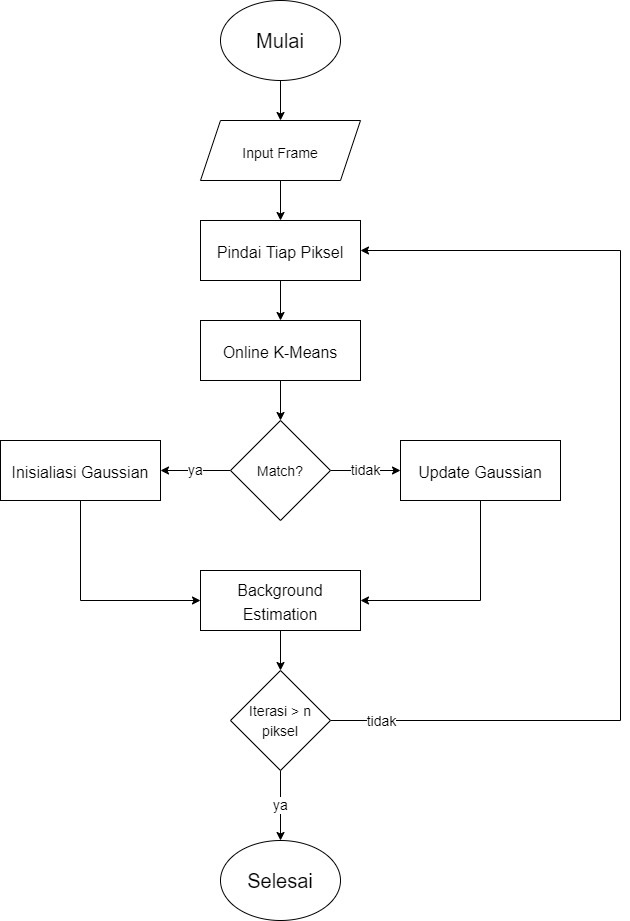
\includegraphics[width=8cm]{image/FlowChart-GMM.jpg}
          \caption{Diagram alir proses \textit{Background Subtraction} dengan GMM}
          \label{fig:gmmflowchart}
        \end{figure}
        
    \subsection{Proses Menghilangkan Noise Melalui Operasi Morfologi}
        Keluaran dari proses deteksi objek menggunakan metode \textit{Background Subtraction} dengan bantuan GMM adalah sebuah citra biner dengan nilai piksel $0$ sebagai latar belakang dan nilai piksel $1$ sebagai latar depan. Citra hasil keluaran proses tersebut masih berisikan banyak \textit{noise} (piksel latar depan yang bukan objek). Maka dari itu, operasi morfologi diperlukan untuk menghilangkan \textit{noise} tersebut.
        \begin{figure}[H]
        \centering
          \singlespacing
          \captionsetup{justification=centering,margin=0.5cm}
          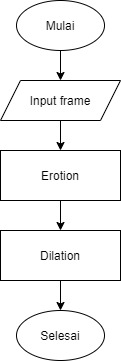
\includegraphics[width=4cm]{image/FlowChart-Morphology.jpg}
          \caption{Diagram alir Operasi Morfologi}
          \label{fig:morphologyflowchart}
        \end{figure}
        
        Citra biner akan melalui dua tahap operasi morfologi, yaitu erosi yang disusul oleh dilasi \textit{(opening)}. Erosi sesuai dengan namanya adalah proses pengikisan piksel. Dalam hal ini, erosi dapat menghilangkan \textit{noise} pada citra biner terutama \textit{salt and pepper noise} (derau kecil pada citra yang terlihat seperti garam bertaburan). \textit{Structuring element} yang akan digunakan oleh proses erosi berukuran $5 \times 5$ dengan bentuk kotak. Proses dilasi selanjutnya dilakukan untuk mengembalikan objek latar depan ke bentuk semula yang sebelumnya terkikis oleh proses erosi. Dilasi dapat memperbesar objek latar depan dan juga menyambungkan kembali bagian-bagian objek yang terpisah akibat proses erosi. \textit{Structuring element} yang akan digunakan oleh proses dilasi berukuran $11 \times 11$ dengan bentuk kotak. Keluaran yang diharapkan adalah citra biner yang bersih dari \textit{noise} serta objek latar depan yang utuh (tidak terpotong ataupun berlubang). Gambar \ref{fig:morphologyflowchart} memperlihatkan diagram alir dari alur operasi morfologi secara keseluruhan.
        
    \subsection{\textit{Downsampling} dan \textit{Contour Tracing}}
        \textit{Downsampling} terhadap sebuah \textit{frame} dijalankan sebelum algoritme CT dieksekusi. Hal ini dilakukan untuk meningkatkan perfoma CT. Algoritme dua dari metode \textit{contour tracing / border following} oleh Suzuki digunakan pada sistem ini. Algoritme dua hanya berfokus pada deteksi tepi bagian terluar \textit{(outer border)}, karena pada sistem kali ini tidak diperlukan deteksi tepi bagian dalam \textit{(hole border)}. Algoritme ini dijalankan dengan asumsi bahwa citra masukan merupakan citra biner dengan piksel bernilai 0 sebagai latar belakang dan piksel bernilai 1 sebagai latar depan (objek).
        
        Masukan berupa citra biner dari proses operasi morfologi yang kemudian dilakukan proses pemindaian \textit{(scan)} mulai dari piksel paling kiri atas. Ketika pemindai sampai pada sebuah piksel $(i, j)$ bernilai $f_{i, j} \neq 0$, ditentukan apakah piksel tersebut merupakan \textit{starting point} dari operasi \textit{border following} untuk tepi luar atau tepi dalam (Gambar \ref{fig:outerandholeborder}). Lalu \textit{parent border} untuk piksel $(i, j)$ ditentukan berdasarkan Gambar \ref{fig:parentborder}. Langkah selanjutnya adalah melakukan operasi \textit{border following} dimulai dari \textit{starting point} piksel $(i, j)$ sampai pointer kembali ke posisi \textit{starting point} (3.e). Dikarenakan algoritme yang digunakan adalah algoritme dua, nilai $NBD$ dan $-NBD$ akan diset masing-masing $2$ dan $-2$. Kemudian \textit{scanner} melanjutkan pemindaian untuk kembali mencari nilai piksel $f_{i, j} \neq 0$. Algoritme dinyatakan selesai apabila \textit{scanner} sudah sampai pada sudut kanan bawah (piksel terakhir).
        \begin{figure}[H]
        \centering
          \singlespacing
          \captionsetup{justification=centering,margin=0.5cm}
          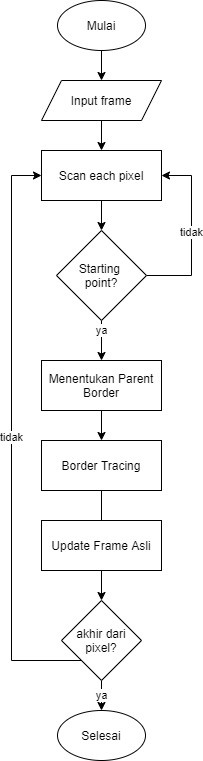
\includegraphics[width=4cm]{image/FlowChart-Countour.jpg}
          \caption{Diagram alir proses \textit{Contour Tracing}}
          \label{fig:countourtracingflowchart}
        \end{figure}
        
        Proses \textit{contour tracing} menghasilkan citra biner yang objek-objeknya sudah mempunyai tepi/konturnya masing-masing. Kemudian dari kontur tersebut dapat diekstraksi lebar dan tinggi sebuah objek. Dari nilai panjang dan lebar  itulah penulis dapat menggambarkan \textit{bounding box} untuk masing-masing objek tersebut.
        
    \subsection{\textit{Decision of Occlusion}, Asosiasi Data, dan Kalman Filter }
        Kalman Filter digunakan sebagai pelacak \textit{(tracker)} untuk masing-masing objek yang terdeteksi. Langkah pertama pada proses pelacakan objek adalah untuk menginisialisasi Kalman Filter sebanyak jumlah objek yang terdeteksi pada proses sebelumnya. Setiap Kalman Filter dikonfigurasikan sebagai berikut:
        \begin{equation}\label{eq:3.1}
        x_k = 
        \begin{bmatrix}
        p_k & q_k & l_k & h_k & v_{p, k} & v_{q, k}
        \end{bmatrix}^T
        \end{equation}
        
        Dimana $p_{k}$ dan $q_{k}$ merepresentasikan nilai horizontal dan vertikal koordinat titik tengah, $l_k$ dan $h_k$ merepresentasikan setengah dari lebar dan tinggi \textit{bounding box}, serta $v_{p, k}$ dan $v_{q, k}$ merepresentasikan kecepatan dari $p_{k}$ dan $q_{k}$.
        
        Kemudian untuk model pengukuran \textit{(measurement model)} yang digunakan oleh sistem ini didefinisikan sebagai berikut:
        \begin{equation}\label{eq:3.2}
        z_k = 
        \begin{bmatrix}
        p_k & q_k & l_k & h_k
        \end{bmatrix}^T
        \end{equation}
        
        Di bawah ini dimodelkan matriks transisi $F$ dan matriks transisi $H$ untuk masing-masing model proses dan model pengukuran:
        \begin{equation}\label{eq:3.3}
        F = 
        \renewcommand{\arraystretch}{1}
        \setlength\arraycolsep{8pt}
        \begin{bmatrix}
        1 & 0 & 0 & 0 & \Delta{t} & 0\\
        0 & 1 & 0 & 0 & 0 & \Delta{t}\\
        0 & 0 & 1 & 0 & 0 & 0\\
        0 & 0 & 0 & 1 & 0 & 0\\
        0 & 0 & 0 & 0 & 1 & 0\\
        0 & 0 & 0 & 0 & 0 & 1
        \end{bmatrix}
        \end{equation}
        
        \begin{equation}\label{eq:3.4}
        H = 
        \renewcommand{\arraystretch}{1}
        \setlength\arraycolsep{9.5pt}
        \begin{bmatrix}
        1 & 0 & 0 & 0 & 0 & 0\\
        0 & 1 & 0 & 0 & 0 & 0\\
        0 & 0 & 1 & 0 & 0 & 0\\
        0 & 0 & 0 & 1 & 0 & 0
        \end{bmatrix}
        \end{equation}
        
        Setelah melalui proses pendefinisian model proses dan model pengukuran di atas, Kalman Filter kemudian dapat digunakan untuk memperkirakan lokasi serta ukuran sebuah objek pada \textit{frame} selanjutnya. Diagram alir untuk proses Kalman Filter dapat dilihat pada Gambar \ref{fig:kalmanfilterflowchart}.
        \begin{figure}[H]
        \centering
          \singlespacing
          \captionsetup{justification=centering,margin=0.5cm}
          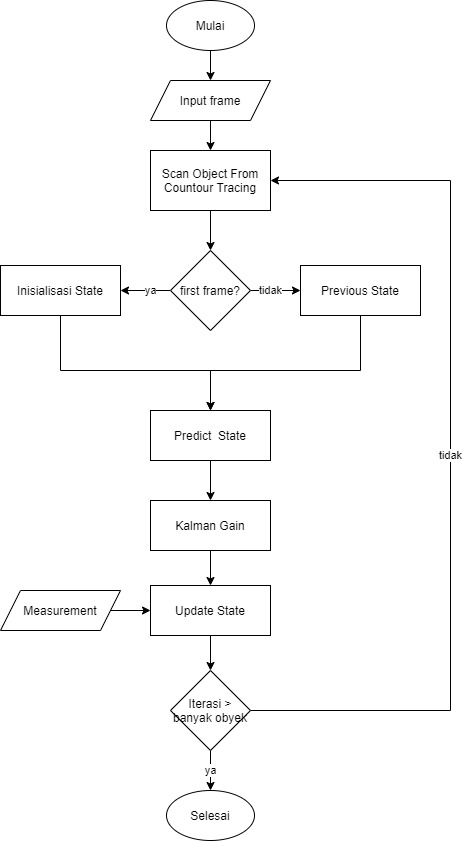
\includegraphics[width=9cm]{image/FlowChart-Kalman Filter.jpg}
          \caption{Diagram alir proses pelacakan dengan Kalman Filter}
          \label{fig:kalmanfilterflowchart}
        \end{figure}
        
        Pada proses ini, Kalman Filter membutuhkan variabel $z_k$ yang didapatkan dari hasil deteksi objek. Untuk menentukan objek hasil deteksi mana yang sesuai dengan prediksi Kalman Filter, dilakukan proses asosiasi data terhadap jarak serta variasi luas antara objek yang diestimasi dengan objek yang dideteksi. Selain itu, proses \textit{decision of occlusion} juga dilakukan untuk menentukan apakah terdapat objek yang mengalami proses \textit{merging} ataupun \textit{splitting}. Setiap objek yang mengalami proses \textit{merging} dengan objek lainnya akan menghasilkan objek baru yang kemudian dipasangkan dengan Kalman Filternya sendiri. Objek baru tersebut akan terus dilacak sampai proses \textit{splitting} terjadi.
        
        \begin{figure}[H]
        \centering
          \singlespacing
          \captionsetup{justification=centering,margin=0.5cm}
          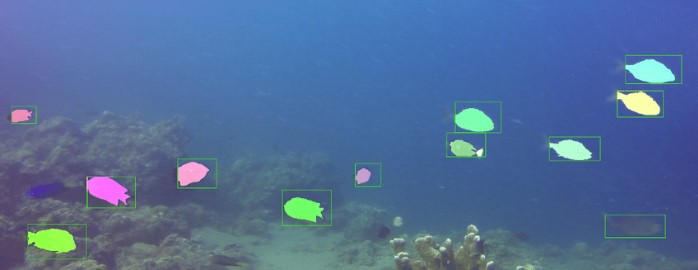
\includegraphics[width=13cm]{image/example_result.jpg}
          \caption{Contoh keluaran sistem}
          \small{Sumber: \href{https://www.researchgate.net/figure/Large-Frame-Fish-Detection-and-Instance-Segmentation_fig1_332153021}{ResearchGate}}
          \label{fig:example_result}
        \end{figure}
        
\section{Perancangan Eksperimen}

    Pada subbab ini akan dibahas mengenai rancangan eksperimen yang akan dilakukan pada penelitian ini. Eksperimen diawali dengan pengambilan data, kemudian dilanjutkan dengan pelacakan oleh sistem, dan terakhir evaluasi hasil.

    \subsection{Sumber Data}
        Berdasarkan sumber datanya, dataset pada penelitian ini akan dibagi menjadi dua. Secara keseluruhan, pengujian dalam penelitian ini dilakukan terhadap video ikan yang sudah direkam sebelumnya \textit{(offline tracking)}. Video tersebut kemudian dimasukkan sebagai input sistem dengan pengaturan bawaan \textit{(default)}. Pengaturan parameter dapat disesuaikan dengan kebutuhan pengguna untuk mendapatkan hasil pelacakan yang optimal.
        
        Dataset didapatkan dari sumber internet. Diunduh dari situs \href{https://alzayats.github.io/DeepFish/}{\textit{DeepFish}} \citep{Saleh2020} dan \href{http://www.perceivelab.com/datasets}{\textit{PeRCeiVeLab}} \citep{Kavasidis2012}. Dataset yang diunduh dari situs \href{https://alzayats.github.io/DeepFish/}{\textit{DeepFish}} berupa kumpulan gambar \textit{frame} video yang kemudian diubah ke dalam bentuk video dengan format mp4 dengan resolusi 720 x 480 dan \textit{frame rate} 24 fps. Sementara itu, dataset yang diunduh dari situs \href{http://www.perceivelab.com/datasets}{\textit{PeRCeiVeLab}} merupakan video dengan format \textit{flv} berdurasi 9 menit dan dengan resolusi 320x240 serta \textit{frame rate} 8 fps. Berdasarkan jumlah ikan dan keadaan latar belakang, terdapat empat skenario pengujian yang akan dilakukan pada penelitian ini. Keempat skenario tersebut adalah:
            \begin{enumerate}
                \item Pengujian terhadap video berisikan satu ikan dengan latar belakang sederhana
                \item Pengujian terhadap video berisikan satu ikan dengan latar belakang kompleks
                \item Pengujian terhadap video berisikan dua atau lebih ikan \textit{(multiple object)} dengan latar belakang sederhana
                \item Pengujian terhadap video berisikan dua atau lebih ikan \textit{(multiple object)} dengan latar belakang kompleks
            \end{enumerate}
        Secara keseluruhan, terdapat empat video yang akan digunakan dalam penelitian ini. Dataset video yang diambil sebagai masukan sistem adalah sebagai berikut:
            \begin{enumerate}
                \item Video skenario pengujian satu diambil dari situs \href{https://alzayats.github.io/DeepFish/}{\textit{DeepFish}} 
                indeks 9908 berdurasi 12 detik (24fps). Video ini digunakan karena latar belakang video termasuk ke dalam kategori sederhana.
                \vspace{-0.5cm}
                \begin{figure}[H]
                \centering
                  \singlespacing
                  \captionsetup{justification=centering,margin=0.5cm}
                  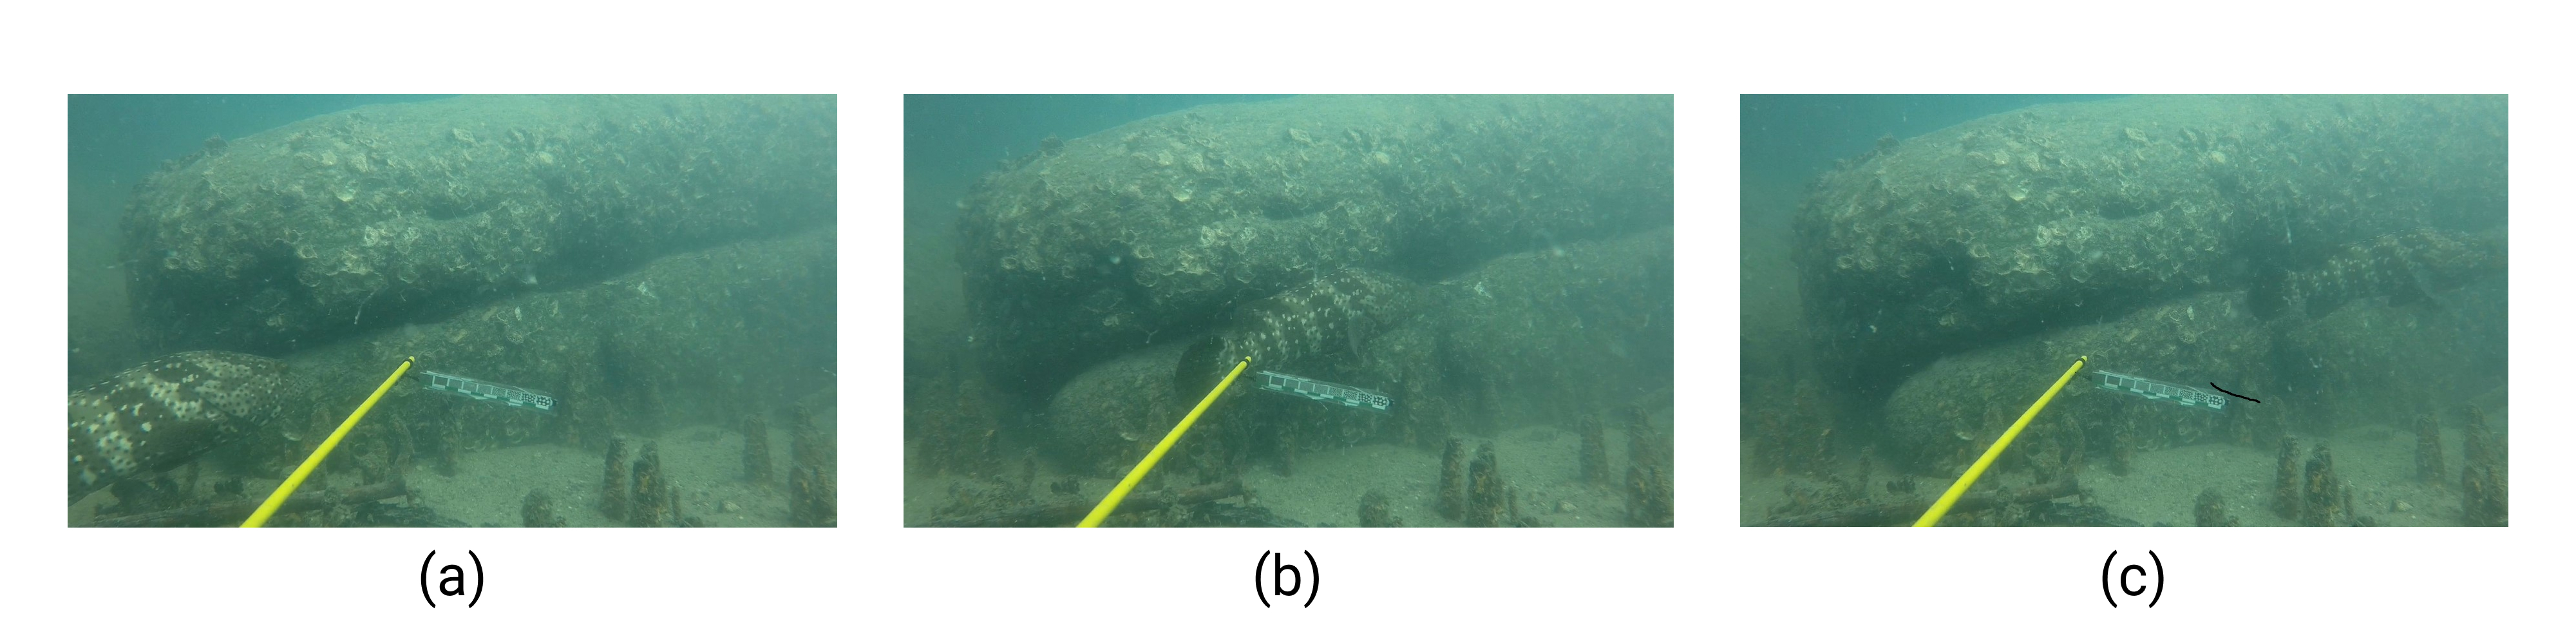
\includegraphics[width=12cm]{image/sample_frame_9908.jpg}
                  \caption{Sampel \textit{frame} video dataset \textit{DeepFish} indeks 9908}
                  \small{Sumber: \href{https://alzayats.github.io/DeepFish/}{\textit{DeepFish Video Dataset}}}
                  \label{fig:sample_9908}
                \end{figure}
                \item Video skenario pengujian dua diambil dari situs \href{https://alzayats.github.io/DeepFish/}{\textit{DeepFish}} 
                indeks 9866 berdurasi 35 detik (24fps). Video ini digunakan karena latar belakang video termasuk ke dalam kategori kompleks (dinamis).
                \vspace{-0.5cm}
                \begin{figure}[H]
                \centering
                  \singlespacing
                  \captionsetup{justification=centering,margin=0.5cm}
                  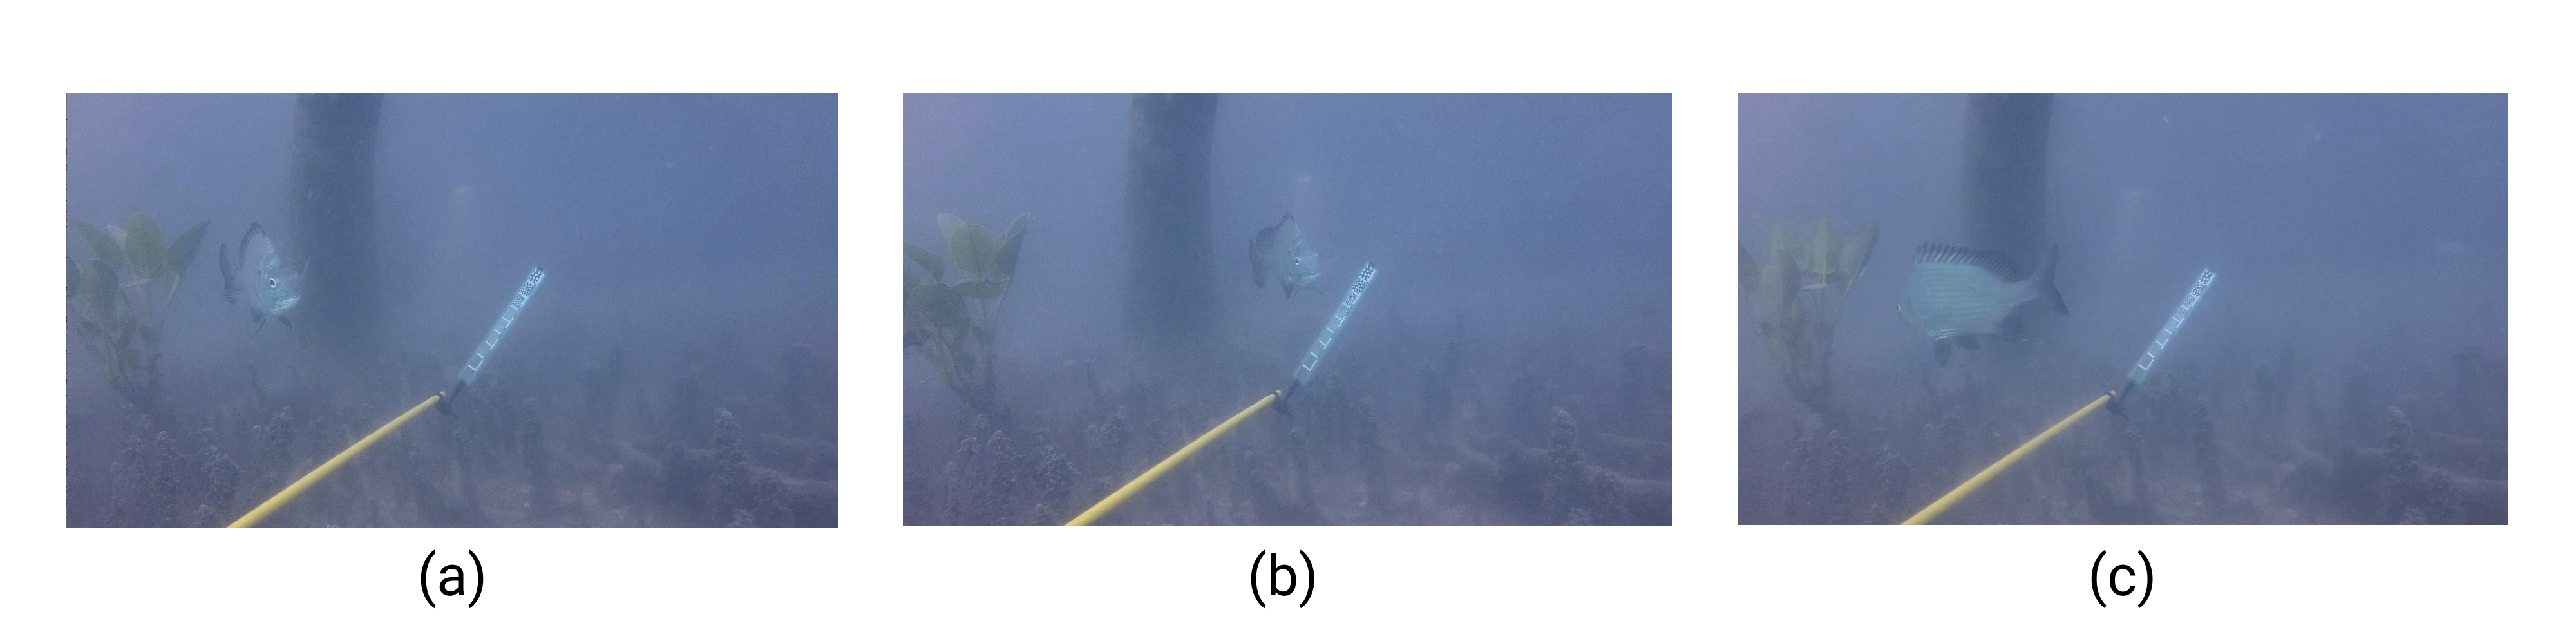
\includegraphics[width=12cm]{image/sample_frame_9866.jpg}
                  \caption{Sampel \textit{frame} video dataset \textit{DeepFish} indeks 9866}
                  \small{Sumber: \href{https://alzayats.github.io/DeepFish/}{\textit{DeepFish Video Dataset}}}
                  \label{fig:sample_9866}
                \end{figure}
                \item Video skenario pengujian tiga diambil dari situs \href{http://www.perceivelab.com/datasets}{\textit{PeRCeiVeLab}}
                indeks gt\textunderscore 124 berdurasi 9 menit 22 detik (8fps) yang telah dipotong menjadi 2 menit 30 detik. Video ini digunakan karena sudah cukup memenuhi kriteria skenario pengujian ke-tiga, yaitu jumlah objek lebih dari satu dengan latar belakang sederhana.
                \vspace{-0.5cm}
                \begin{figure}[H]
                \centering
                  \singlespacing
                  \captionsetup{justification=centering,margin=0.5cm}
                  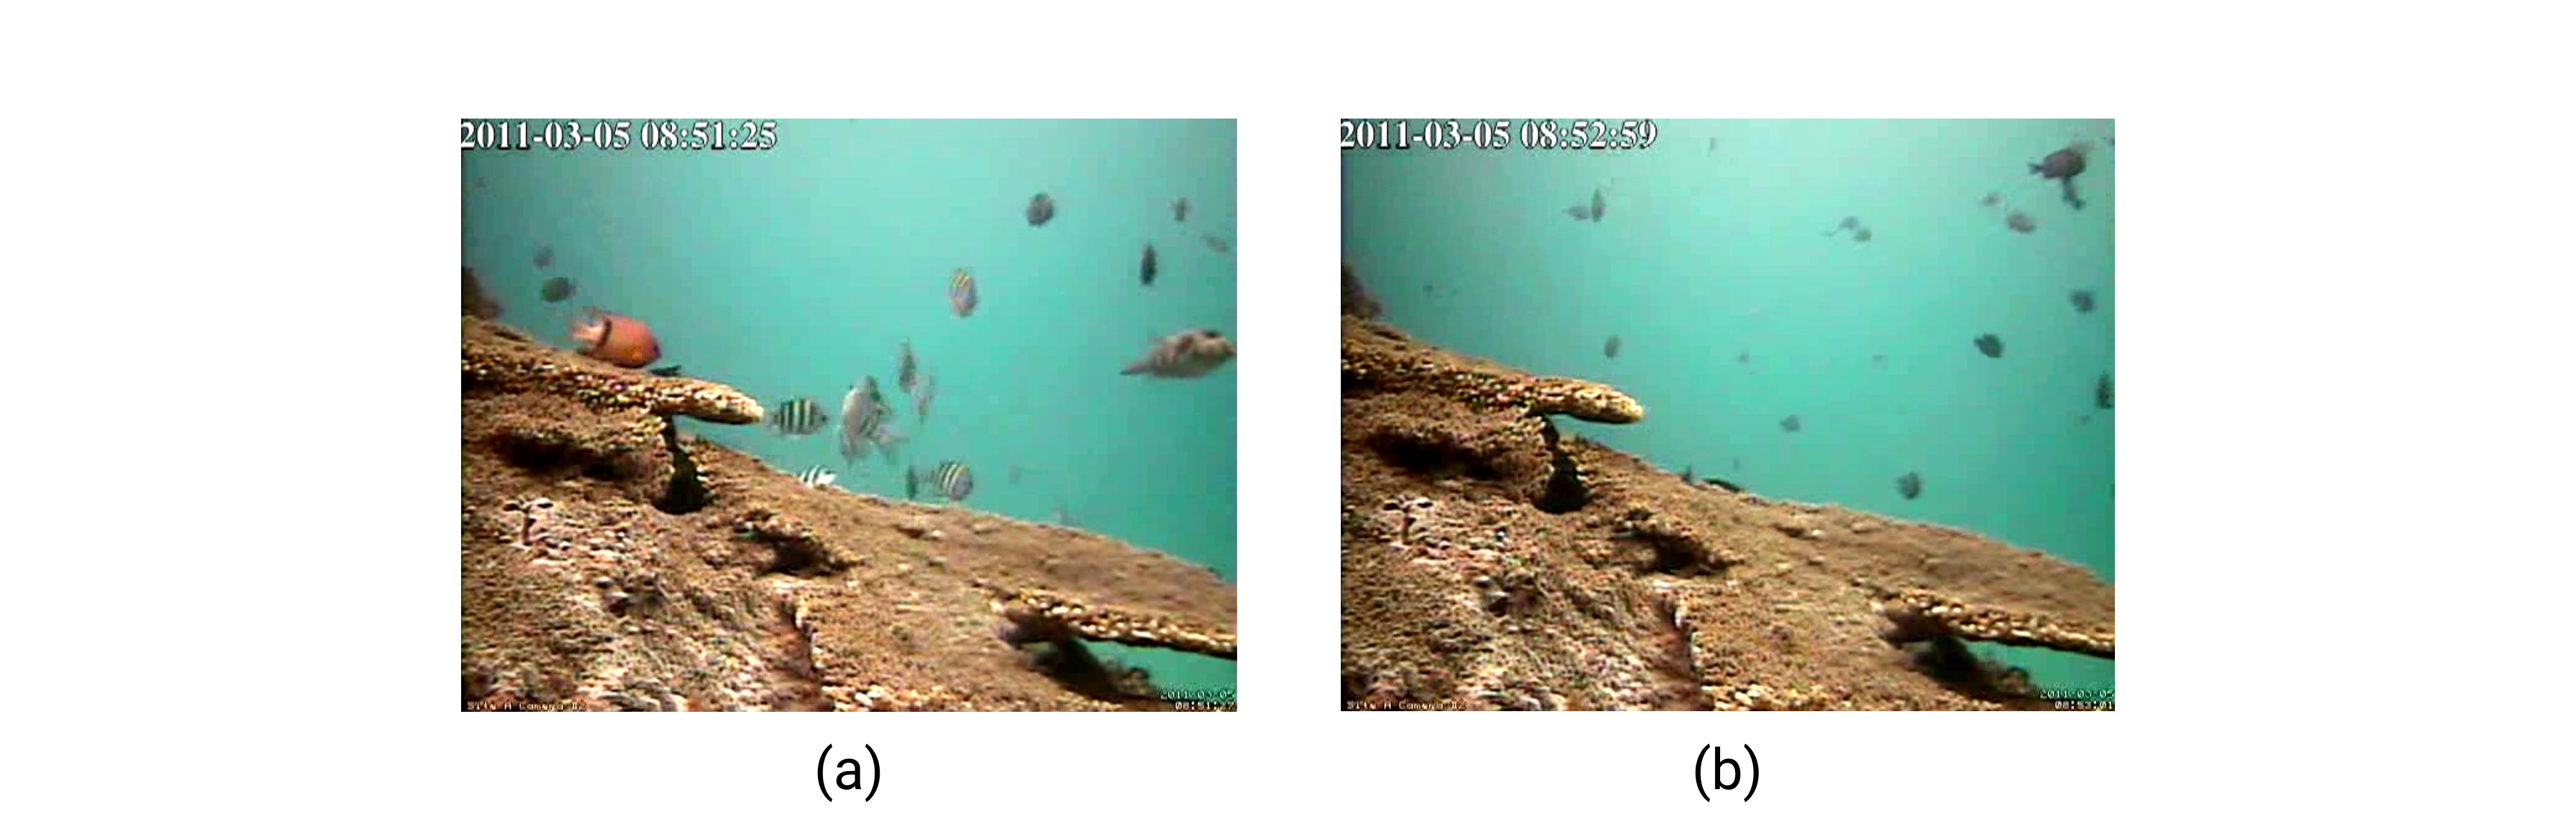
\includegraphics[width=12cm]{image/sample_frame_gt_124.jpg}
                  \caption{Sampel \textit{frame} video dataset \textit{PeRCeiVeLab} indeks gt\textunderscore 124}
                  \small{Sumber: \href{https://alzayats.github.io/DeepFish/}{\textit{DeepFish Video Dataset}}}
                  \label{fig:sample_9866}
                \end{figure}
                \item Video skenario pengujian empat diambil dari situs \href{http://www.perceivelab.com/datasets}{\textit{PeRCeiVeLab}}
                indeks gt\textunderscore 116 berdurasi 9 menit 35 detik (8fps) yang telah dipotong menjadi 2 menit 30 detik. Video ini digunakan karena sudah cukup memenuhi kriteria skenario pengujian ke-empat, yaitu jumlah objek lebih dari satu dengan latar belakang kompleks.
                \vspace{-0.5cm}
                \begin{figure}[H]
                \centering
                  \singlespacing
                  \captionsetup{justification=centering,margin=0.5cm}
                  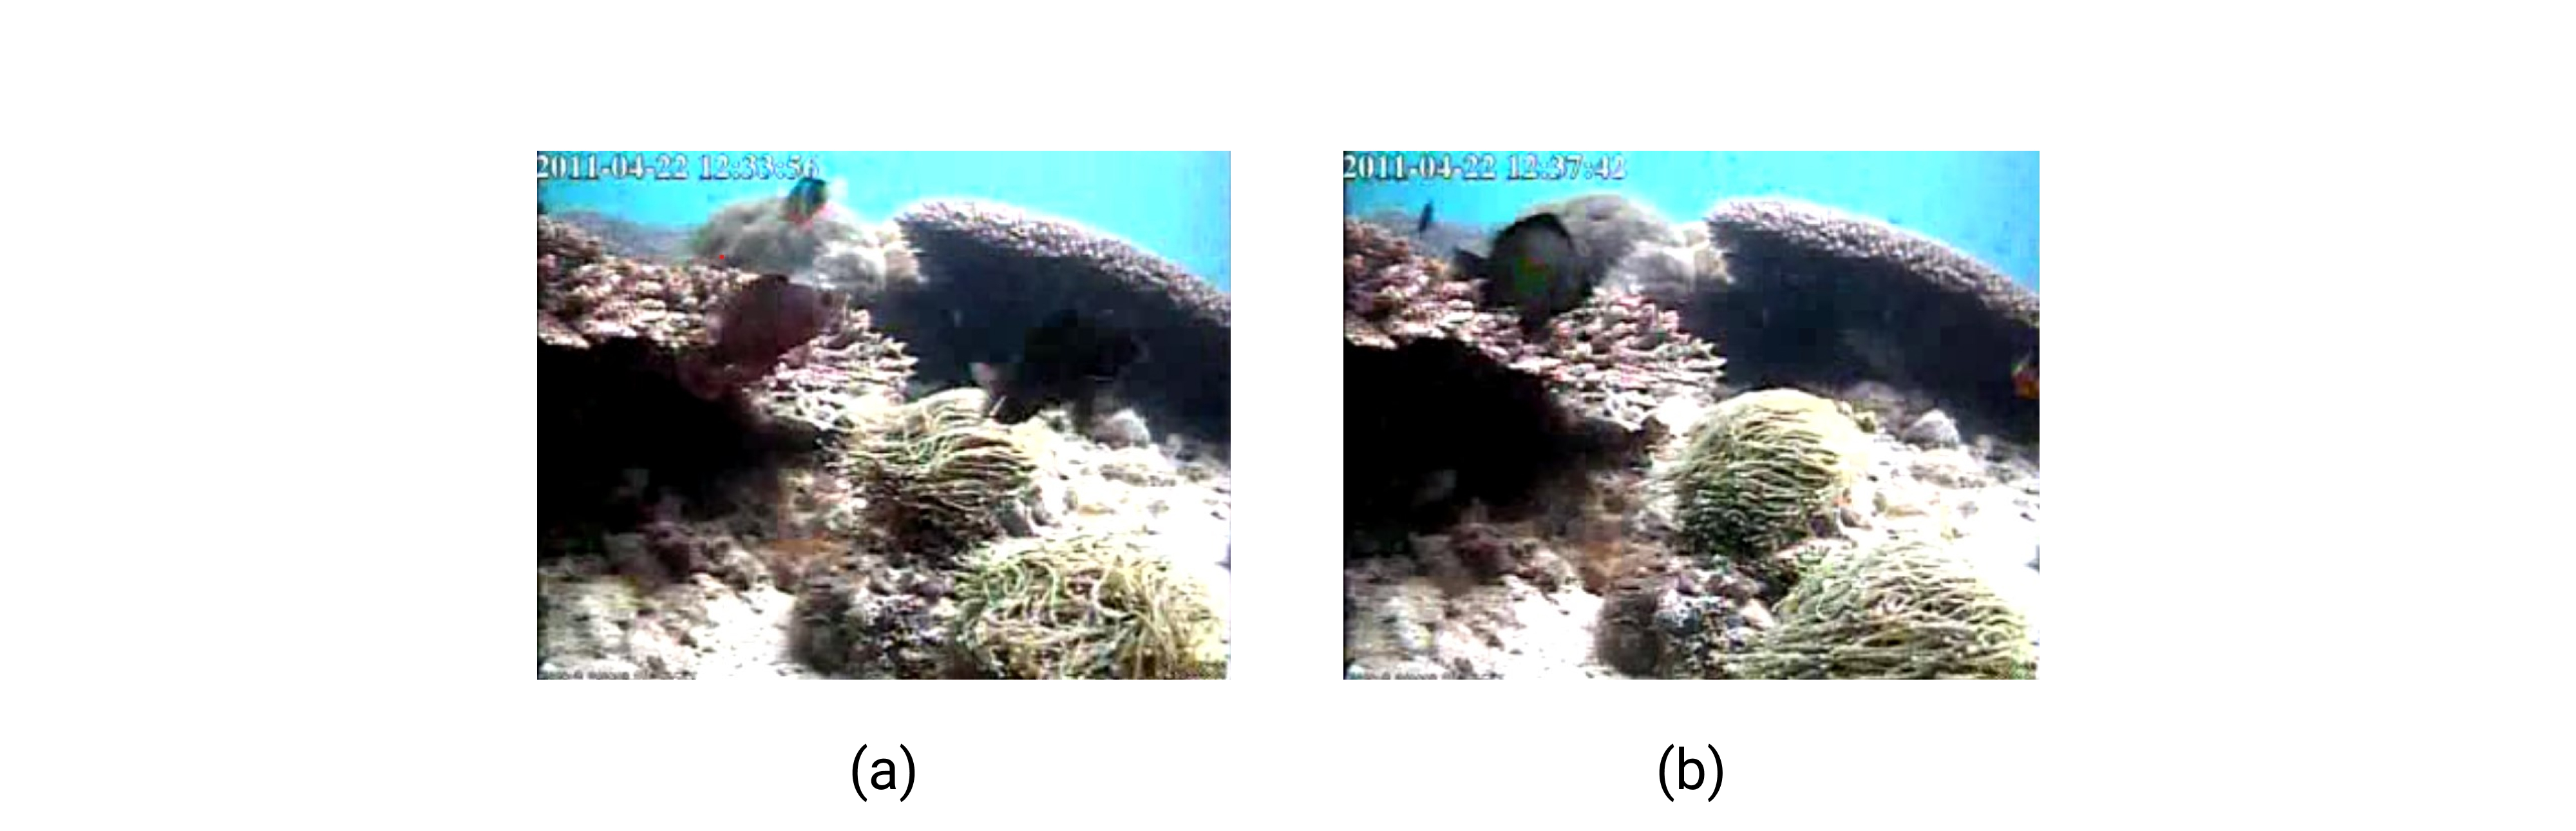
\includegraphics[width=14cm]{image/sample_frame_gt_116.jpg}
                  \caption{Sampel \textit{frame} video dataset \textit{PeRCeiVeLab} indeks gt\textunderscore 116}
                  \small{Sumber: \href{https://alzayats.github.io/DeepFish/}{\textit{DeepFish Video Dataset}}}
                  \label{fig:sample_9866}
                \end{figure}
            \end{enumerate}
        
    \subsection{Evaluasi Hasil}
    Pada subbab ini akan dijelaskan terkait validasi / pembuktian kebenaran dari metode-metode utama pada penelitian ini. Metode-metode tersebut adalah GMM, \textit{Contour Tracing}, dan Kalman Filter. Adapun pembuktian metode-metode tersebut dapat dijabarkan sebagai berikut.
    
        \setlist{ listparindent=\parindent, parsep=0pt}
        \begin{enumerate}
            \item GMM dan Morfologi
            
            Masukan dari metode ini dapat berupa citra RGB ataupun citra biner. Keluaran yang dihasilkan dari metode GMM adalah citra biner dengan piksel bernilai 0 sebagai latar belakang dan piksel bernilai 1 sebagai latar depan (objek). Hasil dari metode ini dapat dikatakan baik apabila ekstraksi latar depan sudah sesuai dengan objek bergerak yang ingin dilacak, dalam kasus ini yaitu objek ikan. Sebaliknya, jika objek selain ikan ikut terekstrak sebagai bagian dari latar depan (latar belakang dinamis, gelembung air), maka sistem dianggap kurang baik.
            
            \begin{figure}[H]
            \centering
              \singlespacing
              \captionsetup{justification=centering,margin=0.5cm}
              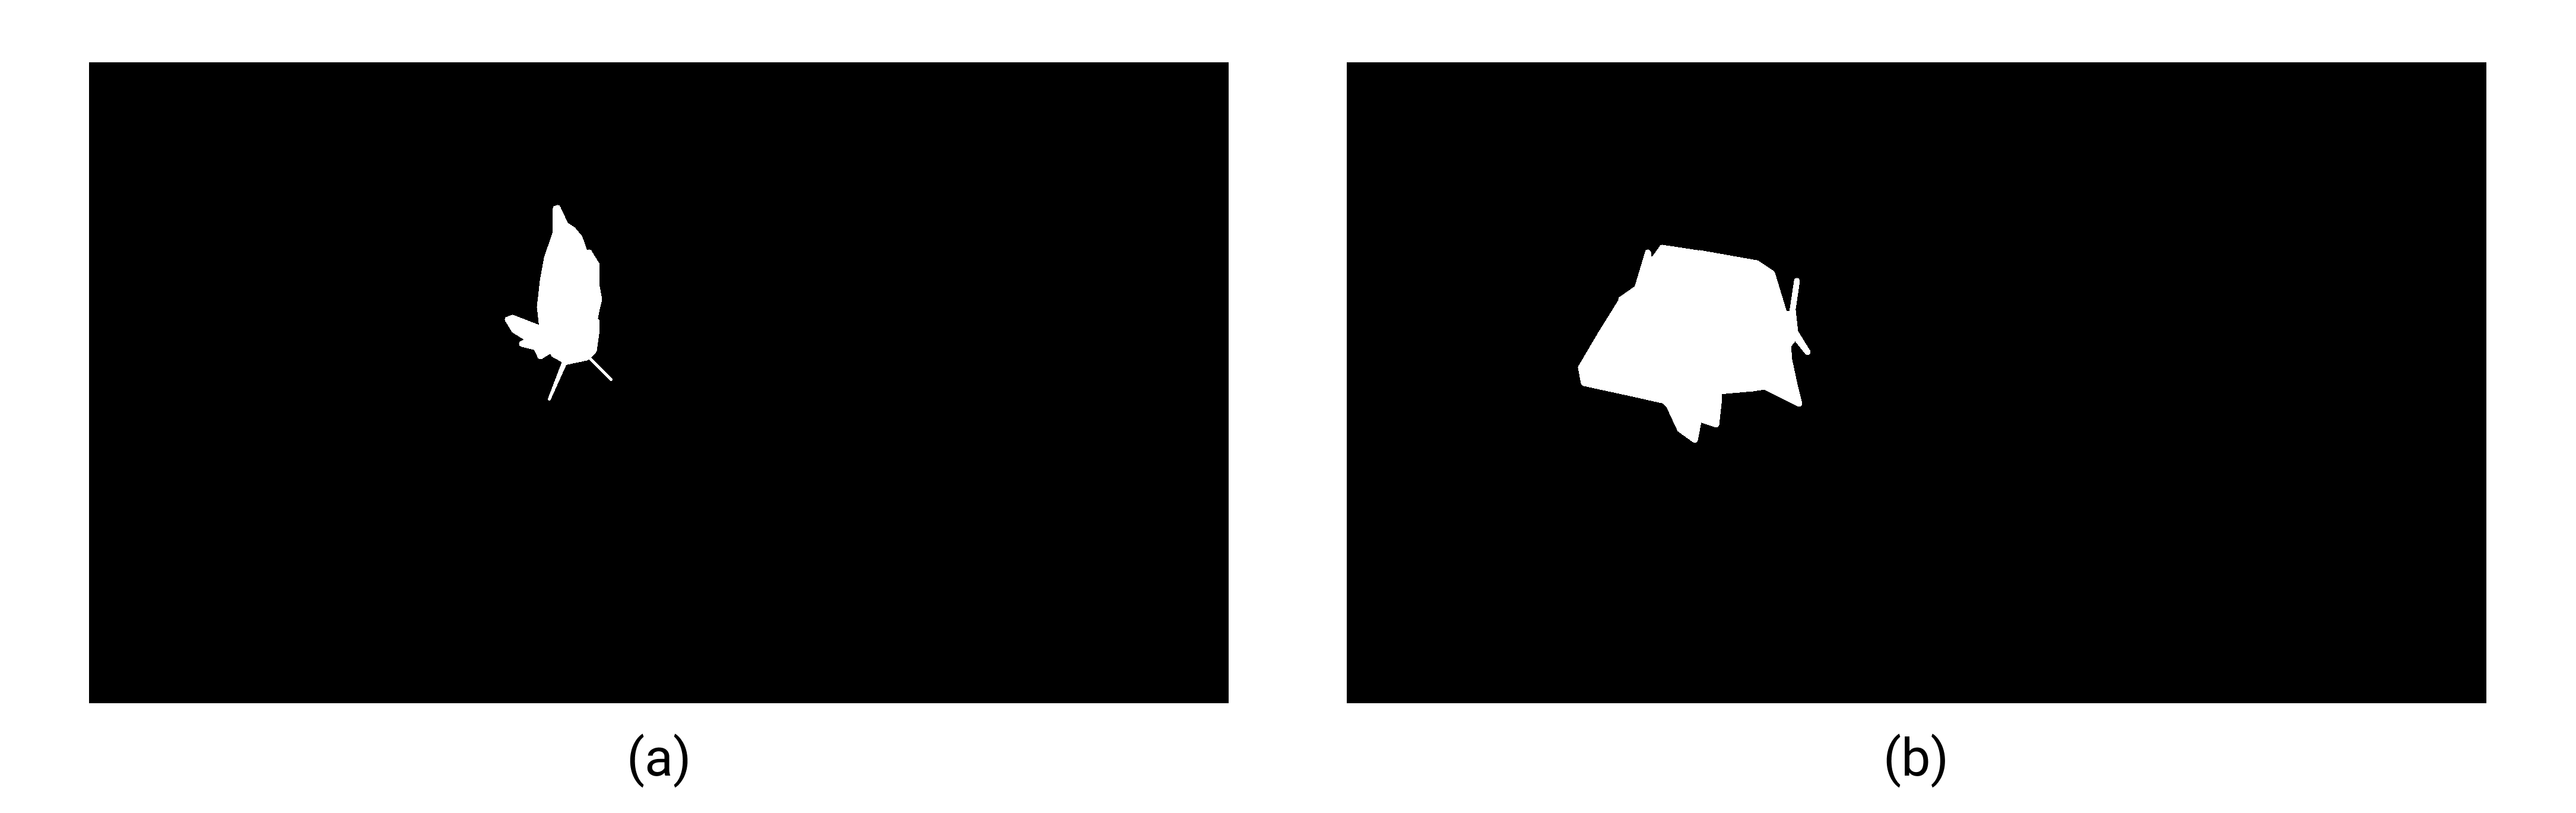
\includegraphics[width=10cm]{image/gt1.jpg}
              \caption{Contoh \textit{groundtruth} GMM}
              \label{fig:gt1}
            \end{figure}
            
            Performa metode GMM dihitung dengan cara membandingkan hasil deteksi objek dengan \textit{groundtruth} (Gambar \ref{fig:gt1}). Sebanyak 3 (tiga) sampel \textit{groundtruth} diambil dari masing-masing video. Empat buah variabel, $A$ \textit{(Accuracy)}, $P$ \textit{(Precision)}, $R$ \textit{(Recall)}, $F1$ \textit{(F1 Score)} dan digunakan untuk mengukur performa metode sebagai berikut:
            
            \begin{equation}\label{eq:3.5}
           	A = \frac{TN + TP}{TN + FP + TP + FN} \times 100 \%
            \end{equation}
            
            \begin{equation}\label{eq:3.5}
            P = \frac{TP}{TP + FP} \times 100 \%
            \end{equation}
            
            \begin{equation}\label{eq:3.6}
            R = \frac{TP}{TP + FN} \times 100 \%
            \end{equation}
        
	        \begin{equation}\label{eq:3.6}
        	F1 = 2 \cdot \frac{P \cdot R}{P + R} \times 100 \%
	        \end{equation}
            
            dimana $A$ merepresentasikan jumlah piksel yang dideteksi dari seluruh deteksi adalah benar latar depan,  $P$ \textit{(Precision)} merepresentasikan seberapa besar persentase piksel yang diprediksi adalah benar latar depan, $R$ \textit{(Recall)} merepresentasikan seberapa besar persentase piksel latar depan yang berhasil dideteksi, $F1$ merupakan gabungan dari \textit{Recall} dan \textit{Precision}, $TP$ \textit{(True Positive)} adalah hasil deteksi piksel latar depan yang benar, $TN$ \textit{(True Negative)} adalah hasil deteksi piksel latar belakang yang benar, $FP$ \textit{(False Positive)} adalah piksel latar belakang yang terdeteksi sebagai piksel latar depan, dan $FN$ \textit{(False Negative)} adalah piksel latar depan yang tidak terdeteksi oleh sistem \citep{Chavan2017}. Performa metode GMM dapat dikatakan baik apabila variabel $P$ dan $R$ menghasilkan nilai persentase yang besar.
            
            \item \textit{Downsampling}

            Metode \textit{Downsapling} diperlukan untuk meningkatkan performa 
            \textit{tracing} pada metode CT dengan memperhitungkan juga akurasi sistem serta kualitas gambar. Tiga $(3)$ buah sampel diambil dari masing-masing video. Evaluasi dihitung dengan cara membandingkan waktu eksekusi metode CT sebelum dan sesudah dilakukan \textit{downsampling} pada \textit{frame} terkait.
            
            \item \textit{Contour Tracing}
            
            Metode CT mengambil masukan citra biner dari proses deteksi objek bergerak sebelumnya. Metode ini menghasilkan citra biner yang setiap objek bergerak sudah mempunyai tepi / konturnya masing-masing. Dari kontur tersebut dapat dihasilkan \textit{bounding box}. Pembuktian dapat dilakukan dengan cara membandingkan jumlah objek / jumlah kontur hasil metode CT dengan \textit{groundtruth}. Sebanyak $3$ (tiga) buah sampel \textit{groundtruth} diambil dari masing-masing video. Dua atau lebih objek yang mengalami proses \textit{occlusion} dapat diklasifikasikan sebagai satu objek. \textit{Absolute Error} digunakan dalam proses evaluasi metode CT.
            \begin{equation}\label{eq:3.7}
            \text{AE} = \bigg|\frac{\textit{Jumlah objek sebenarnya - Jumah objek hasil CT}}{\textit{Jumah objek hasil CT}}\bigg| \times 100\%
            \end{equation}
            
            Nilai $\textit{Absolute Error} =  0\%$ menyatakan bahwa jumlah objek sudah sesuai dengan \textit{groundtruth}. Performa metode CT sangat bergantung pada hasil deteksi objek dari metode sebelumnya. Maka dari itu, jika nilai $\textit{error}$ cukup besar, perlu dilakukan penyesuaian parameter sistem untuk kemudian dilakukan pengujian ulang agar mendapatkan hasil yang baik.
            \begin{figure}[H]
            \centering
              \singlespacing
              \captionsetup{justification=centering,margin=0.5cm}
              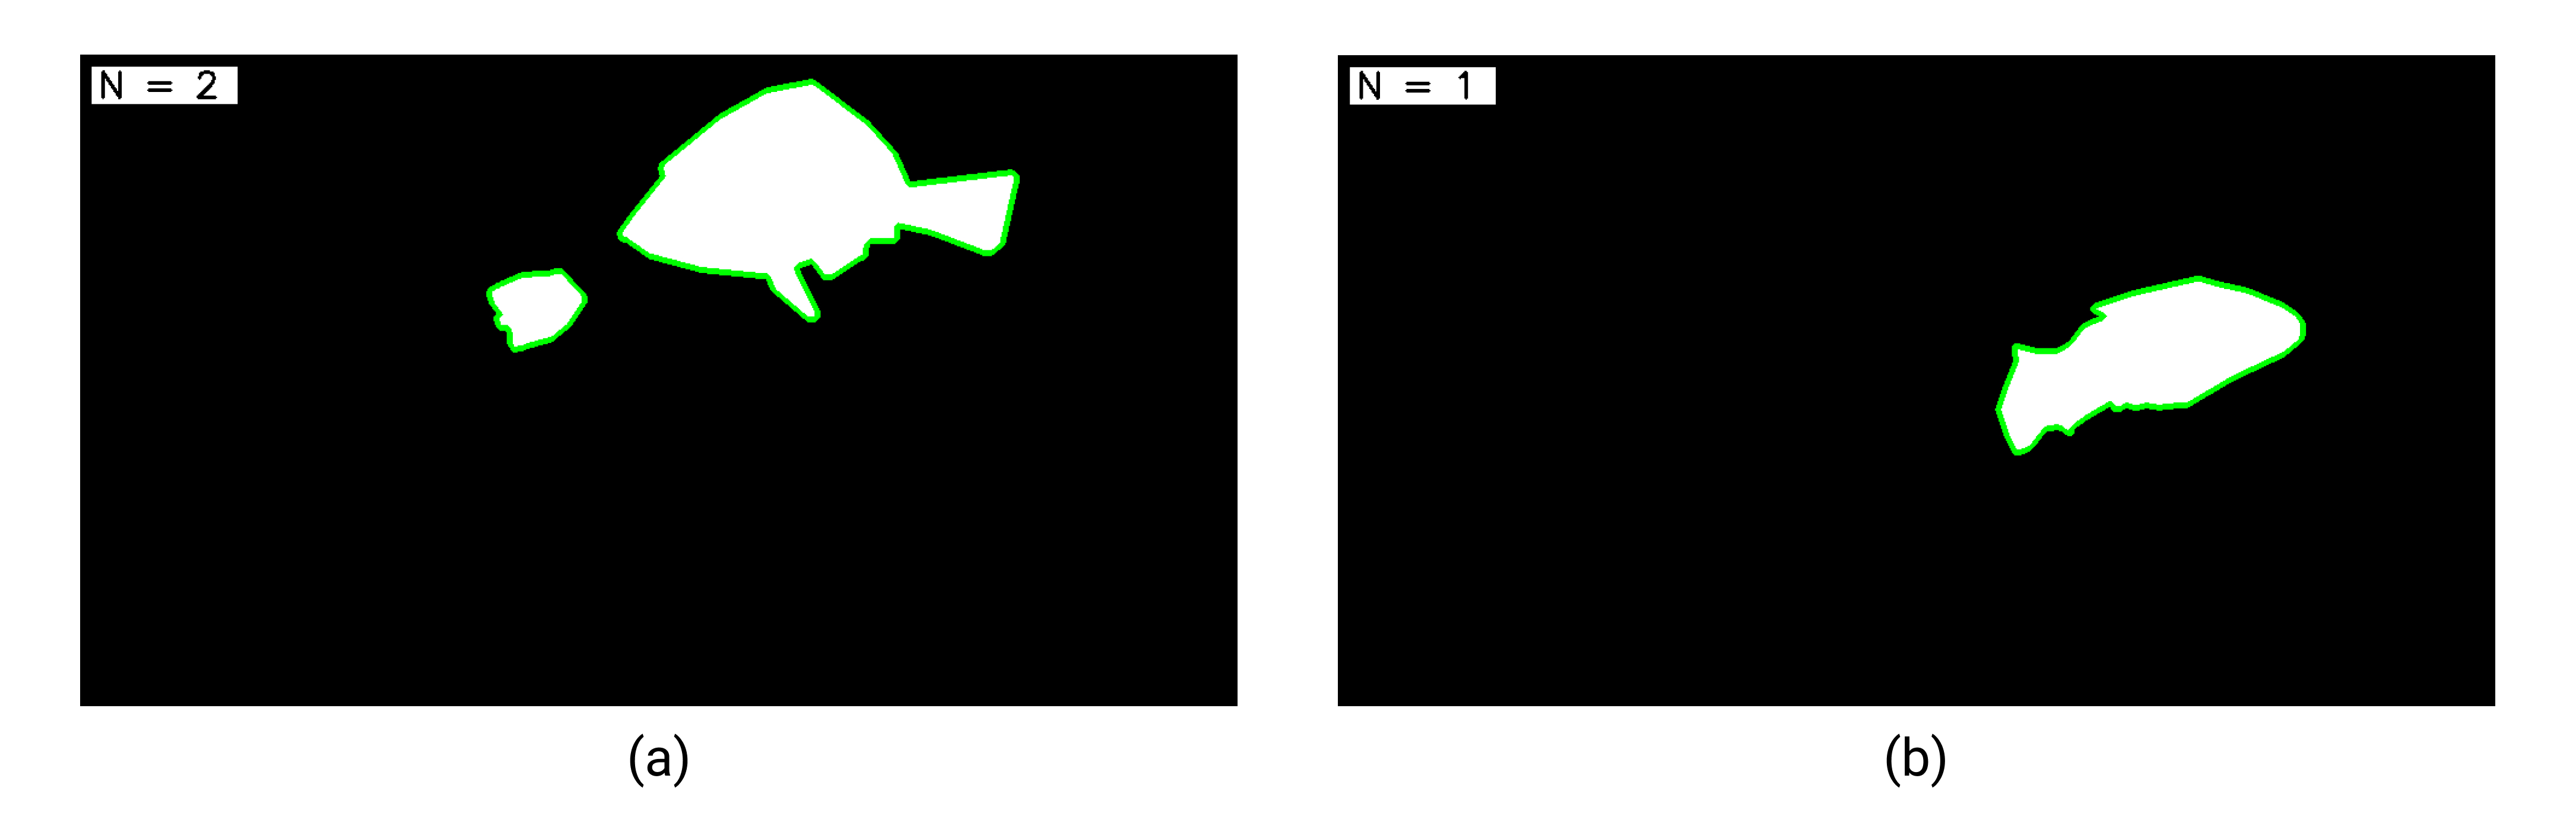
\includegraphics[width=10cm]{image/gt_ct.jpg}
              \caption{Contoh \textit{groundtruth} \textit{Contour Tracing}}
              \label{fig:gt1}
            \end{figure}
            
            \item Pelacakan Objek dengan Kalman Filter
            
            Kalman Filter bertugas sebagai pemberi label/identitas untuk setiap objek yang mempunyai \textit{bounding box}. Proses asosiasi data membuat Kalman Filter dapat mempertahankan label masing-masing objek tersebut selama video berlangsung. Inilah yang disebut sebagai proses "pelacakan objek". Keluaran dari proses ini adalah \textit{running} video berisikan objek yang dilacak lengkap dengan \textit{bounding box} serta label uniknya masing-masing. 
            
            Performa metode Kalman Filter dihitung dengan cara membandingkan hasil pelacakan oleh sistem dengan \textit{groundtruth} berupa koordinat nilai tengah masing-masing objek. Sampel \textit{groundtruht} diambil dari masing-masing video sebanyak 3 sampel. \textit{Root Mean Squared Error} \textit{(RMSE)} digunakan untuk mengukur performa nilai yang diprediksi oleh  model \textit{(predicted)} dengan nilai sebenarnya \textit{(observed)}. Formula \textit{RMSE} dapat didefinisikan sebagai berikut: 
            \begin{equation}\label{eq:3.8}
            \textit{TOTAL RMSE} = \sqrt{(RMSE_X)^2 + (RMSE_Y)^2}
            \end{equation}
            dimana
            \begin{equation}\label{eq:3.9}
            RMSE_X = \sqrt{\sum_{i = 1}^n  \frac{(\hat{x}_i - x_i)^2}{n}}
            \end{equation}
            \begin{equation}\label{eq:3.10}
            RMSE_Y = \sqrt{\sum_{i = 1}^n  \frac{(\hat{y}_i - y_i)^2}{n}}
            \end{equation}
            
            Variabel $\hat{x}_i$, $\hat{y}_i$ adalah nilai koordinat titik tengah $(x, y)$ yang diprediksi, sementara $x_i$, $y_i$ adalah nilai koordinat titik tengah $(x, y)$ yang diobservasi, dan $n$ adalah jumlah observasi. Hasil pelacakan dapat dikatakan baik apabila nilai \textit{TOTAL RMSE} mendekati 0.
        \end{enumerate}
    
    \subsection{Parameter Sistem}
    
    Dalam sistem pelacakan ini, terdapat beberapa parameter yang perlu diatur demi mendapatkan hasil pelacakan yang optimal. Pengujian \textit{tuning} parameter dilakukan terhadap seluruh skenario pengujian masing-masing metode pada subbab sebelumnya.
        \begin{enumerate}
            \item \textit{Downsampling Scale}
            
            Besaran skala dalam proses \textit{Downsampling} berfungsi sebagai penentu seberapa besar sistem akan melakukan \textit{Downsampling} terhadap sebuah \textit{frame} sebelum dilakukannya proses \textit{Contour Tracing}. Besaran skala yang digunakan adalah $S = 2,\, 4,\, 8$. Dengan mempertimbangkan kualitas gambar yang dihasilkan dan juga akurasi metode, penentuan besaran skala ini diharapkan dapat meningkatkan performa sistem secara signifikan.
            
            \item Ukuran \textit{Structuring Element}
            
            Terdapat dua \textit{structuring element} yang digunakan pada operasi morfologi. Ukuran bawaan \textit{structuring element} proses erosi adalah $5 \times 5$. Semakin besar ukurannya maka semakin banyak \textit{salt-pepper noise} yang hilang, akan tetapi semakin banyak pula piksel \textit{foreground} yang terkikis. Sementara itu,  ukuran bawaan \textit{structuring element} proses dilasi adalah $7 \times 7$. Semakin besar ukurannya, maka akan semakin baik sistem dalam menyambungkan bagian objek yang terputus ataupun berlubang, akan tetapi semakin besar juga kemungkinan dua buah objek yang seharusnya terpisah menjadi satu.
        \end{enumerate}
    
        
    
% \section{Jadwal Kegiatan}
% 	Quo no atqui omnesque intellegat, ne nominavi argumentum quo. Eum ei purto oporteat dissentiet, soleat utamur an sit. Et assum dicam interpretaris quo. Cetero alterum ea vel, no possit alterum utroque nec. His fuisset quaestio ad. Has eu tritani incorrupte consequuntur, esse aliquip nec ne \ref{jadwal}.

% 	% Please remember to add \use{multirow} to your document preamble in order to suppor multirow cells
% 		\begin{table}[H]
% 		\centering
% 		\caption{Jadwal Penelitian.}
% 		\label{jadwal}
% 		\begin{tabular}{|c|l|l|l|l|l|l|l|}
% 		\hline
% 		\multirow{2}{*}{No} & \multirow{2}{*}{Keterangan} & \multicolumn{6}{c|}{Bulan}                                                                                                                          \\ \cline{3-8} 
% 		                    &                             & 1 & 2 & 3 & 4 & 5 & 6 \\ \hline
% 		1                   & Studi literatur                                  &\cellcolor{gray} &\cellcolor{gray}&                        &                        &                        &                         \\ \hline
% 		2                   & Desain                                           &                        &\cellcolor{gray}&\cellcolor{gray}&                        &                        &                         \\ \hline
% 		3                   & Pembelian bahan                                  &                        &                        &\cellcolor{gray}&                        &                        &                         \\ \hline
% 		4                   & Pembuatan prototipe                              &                        &                        &\cellcolor{gray}&\cellcolor{gray}&\cellcolor{gray}&                         \\ \hline
% 		5                   & Uji coba dan perbaikan                           &                        &                        &                        &\cellcolor{gray}&\cellcolor{gray}&                         \\ \hline
% 		6                   & Penulisan skripsi                                &                        &                        &                        &                        &                        &\cellcolor{gray}\\ \hline
% 		\end{tabular}
% 		\end{table}
	
% Baris ini digunakan untuk membantu dalam melakukan sitasi
% Karena diapit dengan comment, maka baris ini akan diabaikan
% oleh compiler LaTeX.
\begin{comment}
\bibliography{daftar-pustaka}
\end{comment}
